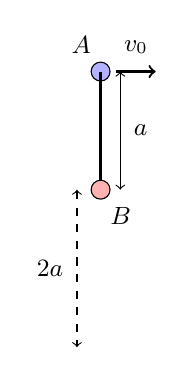
\begin{tikzpicture}[scale=1, font=\small]
  % Problem 5-10: Two balls A, B on rope of length 2a, B below A by distance a
  % Ball A
  \filldraw[fill=blue!30] (0, 2) circle (0.12);
  \node[above left] at (0, 2.1) {$A$};

  % Velocity arrow
  \draw[->, thick] (0.2, 2) -- (0.7, 2);
  \node[above] at (0.45, 2.1) {$\pmb{v}_0$};

  % Rope
  \draw[thick] (0, 2) -- (0, 0.5);

  % Ball B (distance a below A)
  \filldraw[fill=red!30] (0, 0.5) circle (0.12);
  \node[below right] at (0, 0.4) {$B$};

  % Distance a between A and B
  \draw[<->] (0.25, 0.5) -- (0.25, 2);
  \node[right] at (0.3, 1.25) {$a$};

  % Rope length 2a
  \draw[<->, dashed] (-0.3, 0.5) -- (-0.3, -1.5);
  \node[left] at (-0.35, -0.5) {$2a$};
\end{tikzpicture}
